%======================================================================
\subsection{BW-UIX-12 --- Plan: the property inspector in the Browser (23 Oct 2026; built 24 Oct; redesign part-built 24 Oct)}\label{sec:uix12-plan}
%======================================================================

\eref{UIX-12} replaces the \emph{View} and \emph{Data} tabs at the bottom of the Browser with an \emph{inspector}:
a short, grouped card for whatever is selected (a feature, a face, a body or a part), with FreeCAD's full property
editor one click away. The acceptance stays as written: \emph{Pad, Pocket and Fillet edited from the inspector
without the Data tab.} A spike in this build (below) showed it can be done in Python, without C++.

\paragraph{Your answers (23 Oct).}
\begin{center}
\small
\begin{tabularx}{\linewidth}{@{}lX@{}}
\toprule
Question & Answer\\
\midrule
Where & \textbf{In the Browser card}, in place of the View/Data tabs at its bottom (the Browser is the overlay
  model tree: \file{BruceWorx.py} floats it, \file{bruceworx\_browser.py} adds the header and badges).\\
What it shows & The selection: a feature, a face, a body or a part. Size, position, appearance, and the part data,
  including the Heuretes FreeCAD part properties (\S\ref{sec:partprops}).\\
FreeCAD's editor & Stays, one click away (\emph{All properties}), for everything the inspector leaves out.\\
Look & The Browser's transparent mode has no card now (the Nxt look); the inspector must work there too.\\
\bottomrule
\end{tabularx}
\end{center}

\begin{figure}[!htbp]
\centering
\begin{tikzpicture}
  \node[anchor=south west,inner sep=0] (img) at (0,0) {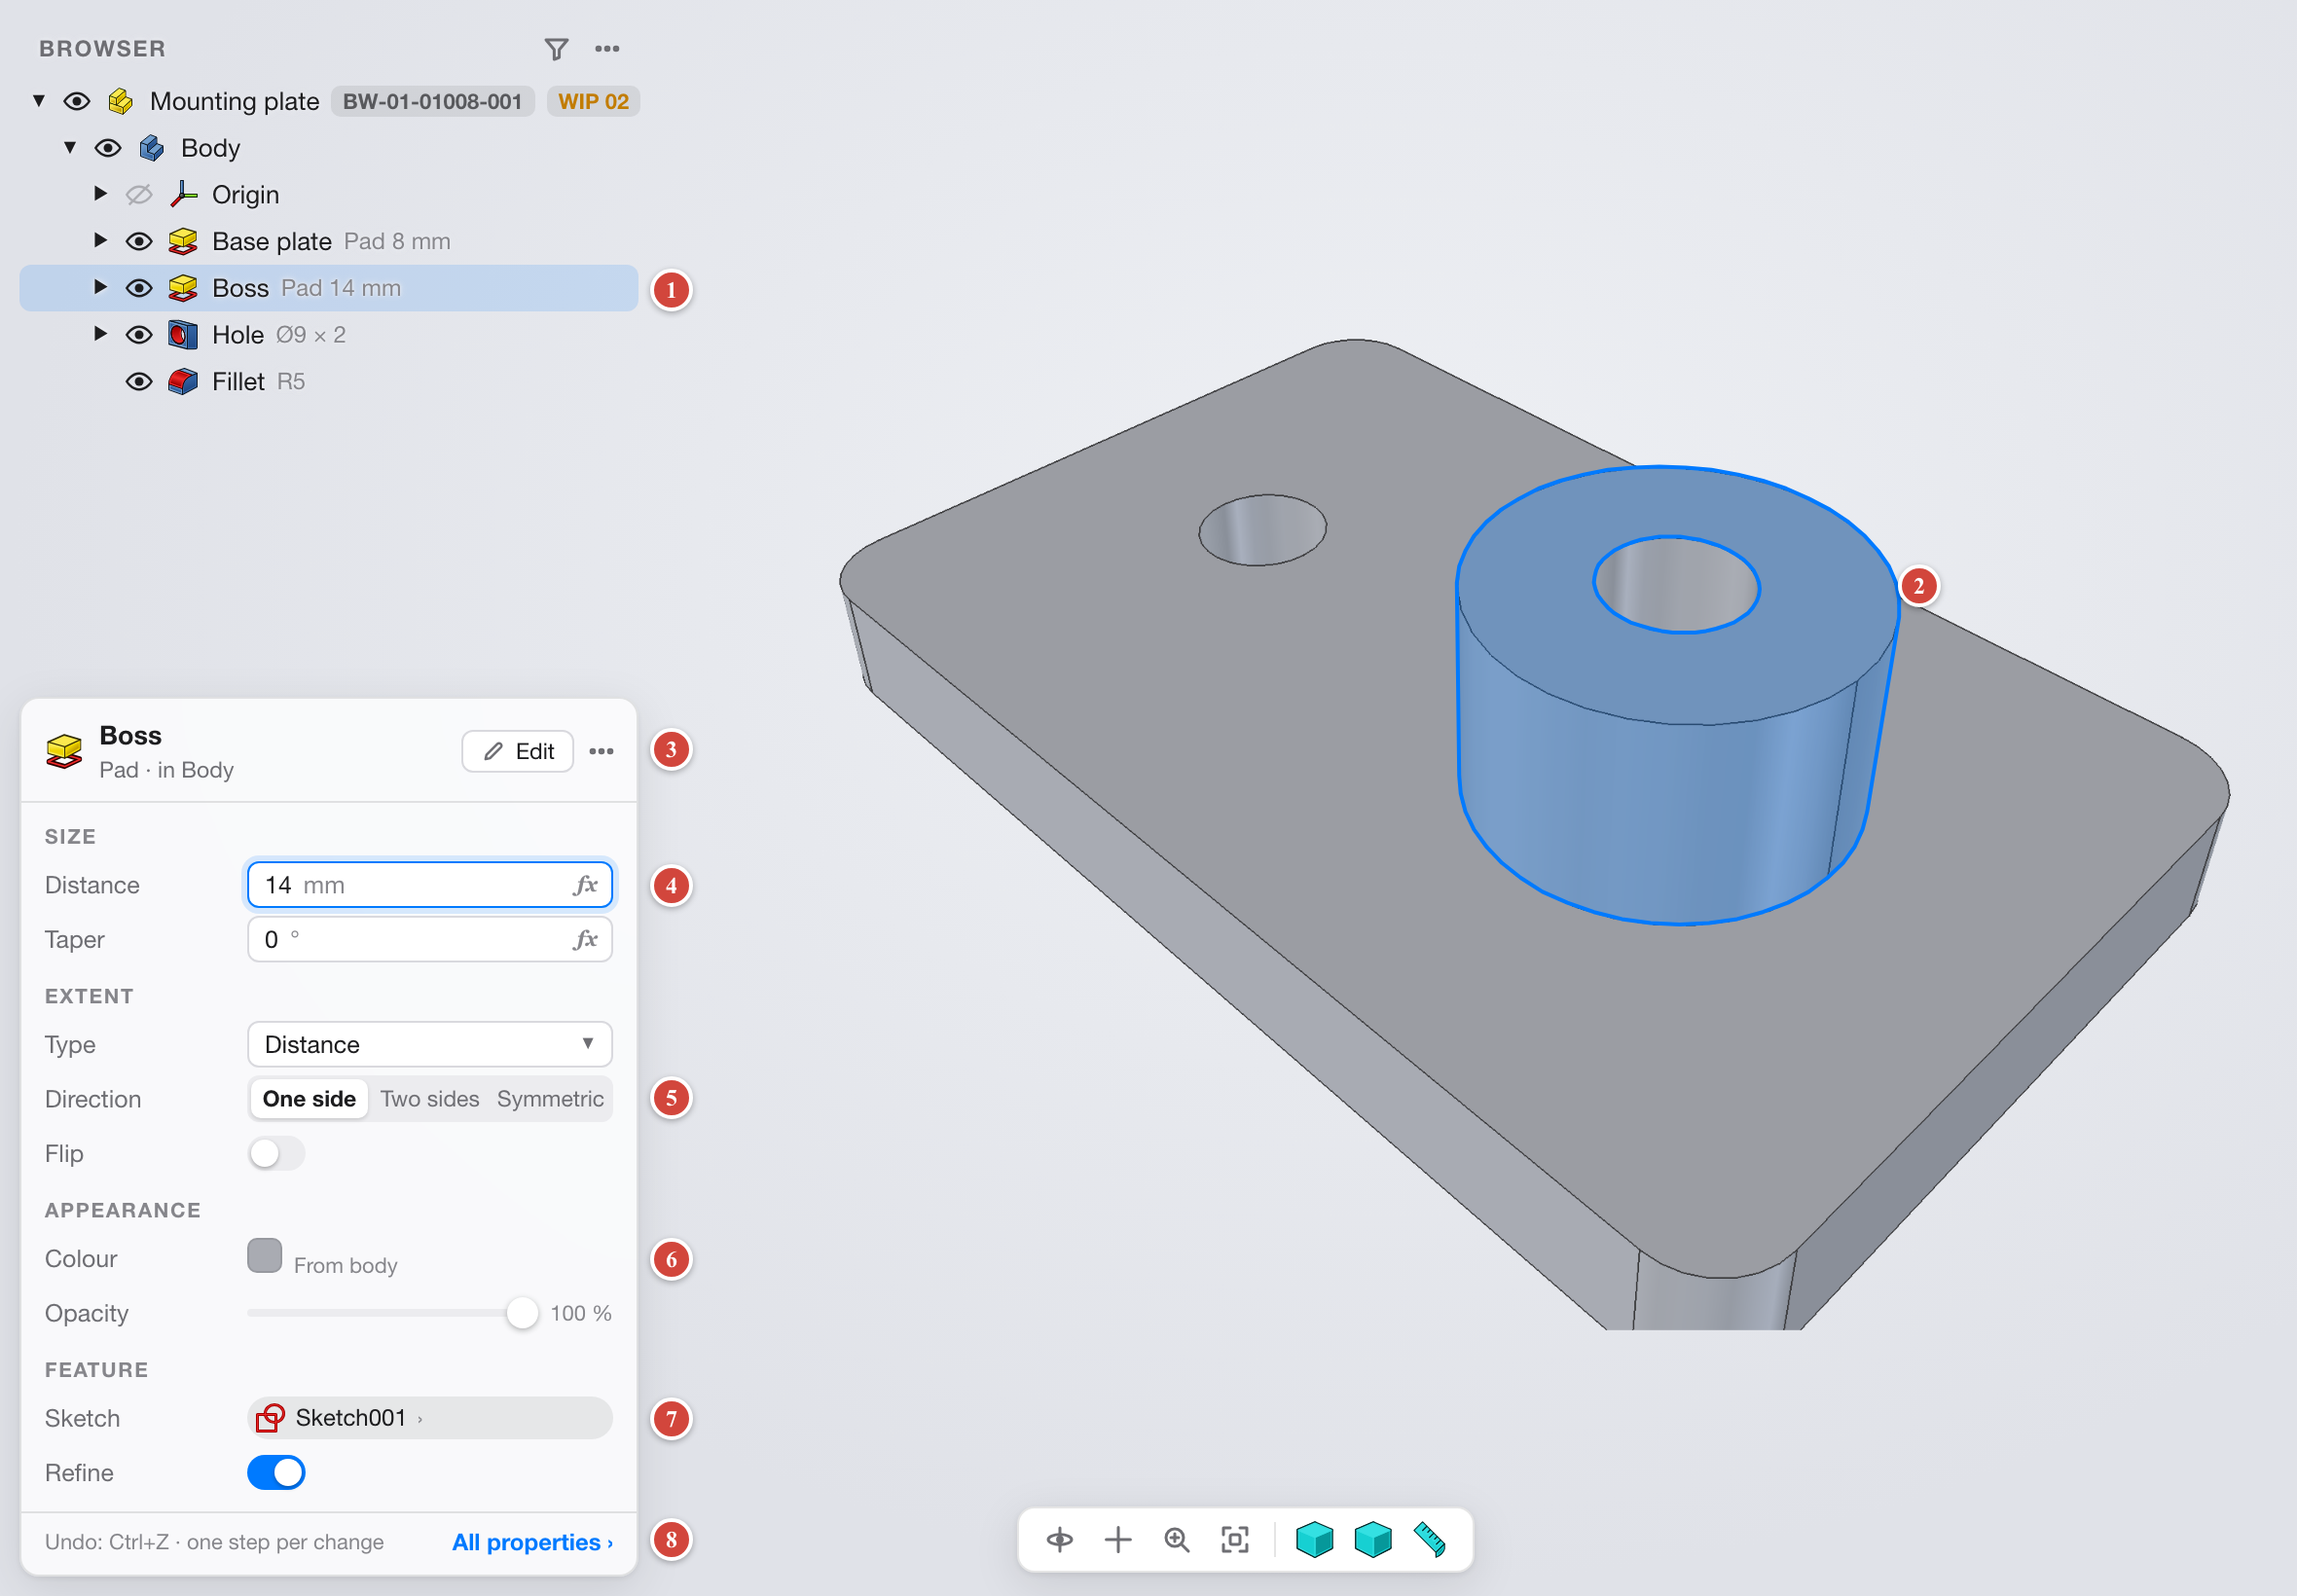
\includegraphics[width=\linewidth]{fig/uix12_browser_notes.png}};
\end{tikzpicture}
\caption{The inspector in the Browser (mock, light). The Boss pad is selected in the Browser; its faces are
highlighted in the view. The numbers match the table below.}
\label{fig:uix12-notes}
\end{figure}

\begin{center}
\small
\begin{tabularx}{\linewidth}{@{}cp{3.2cm}X@{}}
\toprule
\# & Element & Behaviour\\
\midrule
\marker{1} & Selection & Click in the Browser or the view. The tree stays transparent over the model (the Nxt look).\\
\marker{2} & Highlight & The faces of the selected feature, traced through FreeCAD's element map (\eref{UIX-11}).\\
\marker{3} & Header & Icon, name, type and where it lives (``Pad $\cdot$ in Body''). \emph{Edit} opens the feature's own
  task dialog (with FreeCAD~1.1's draggers); $\cdots$ holds Rename, Suppress, Show in property editor.\\
\marker{4} & \textsc{Size} & The feature's dimensions as unit fields with an $f(x)$ button (expressions work as in the Data tab).\\
\marker{5} & \textsc{Extent} & Modes as a segmented control when there are three or fewer choices, otherwise a menu; flags as switches.\\
\marker{6} & \textsc{Appearance} & Colour (or ``from body'' / ``from material'') and opacity.\\
\marker{7} & \textsc{Feature} & Links (profile sketch, base) as chips that select the linked object; Refine.\\
\marker{8} & \emph{All properties} & Swaps the card for FreeCAD's View/Data editor, which gets a \emph{$\langle$ Inspector}
  button to come back. The choice is remembered.\\
\bottomrule
\end{tabularx}
\end{center}

\begin{figure}[!htbp]
\centering
\IfFileExists{fig/uix12_browser_dark.png}{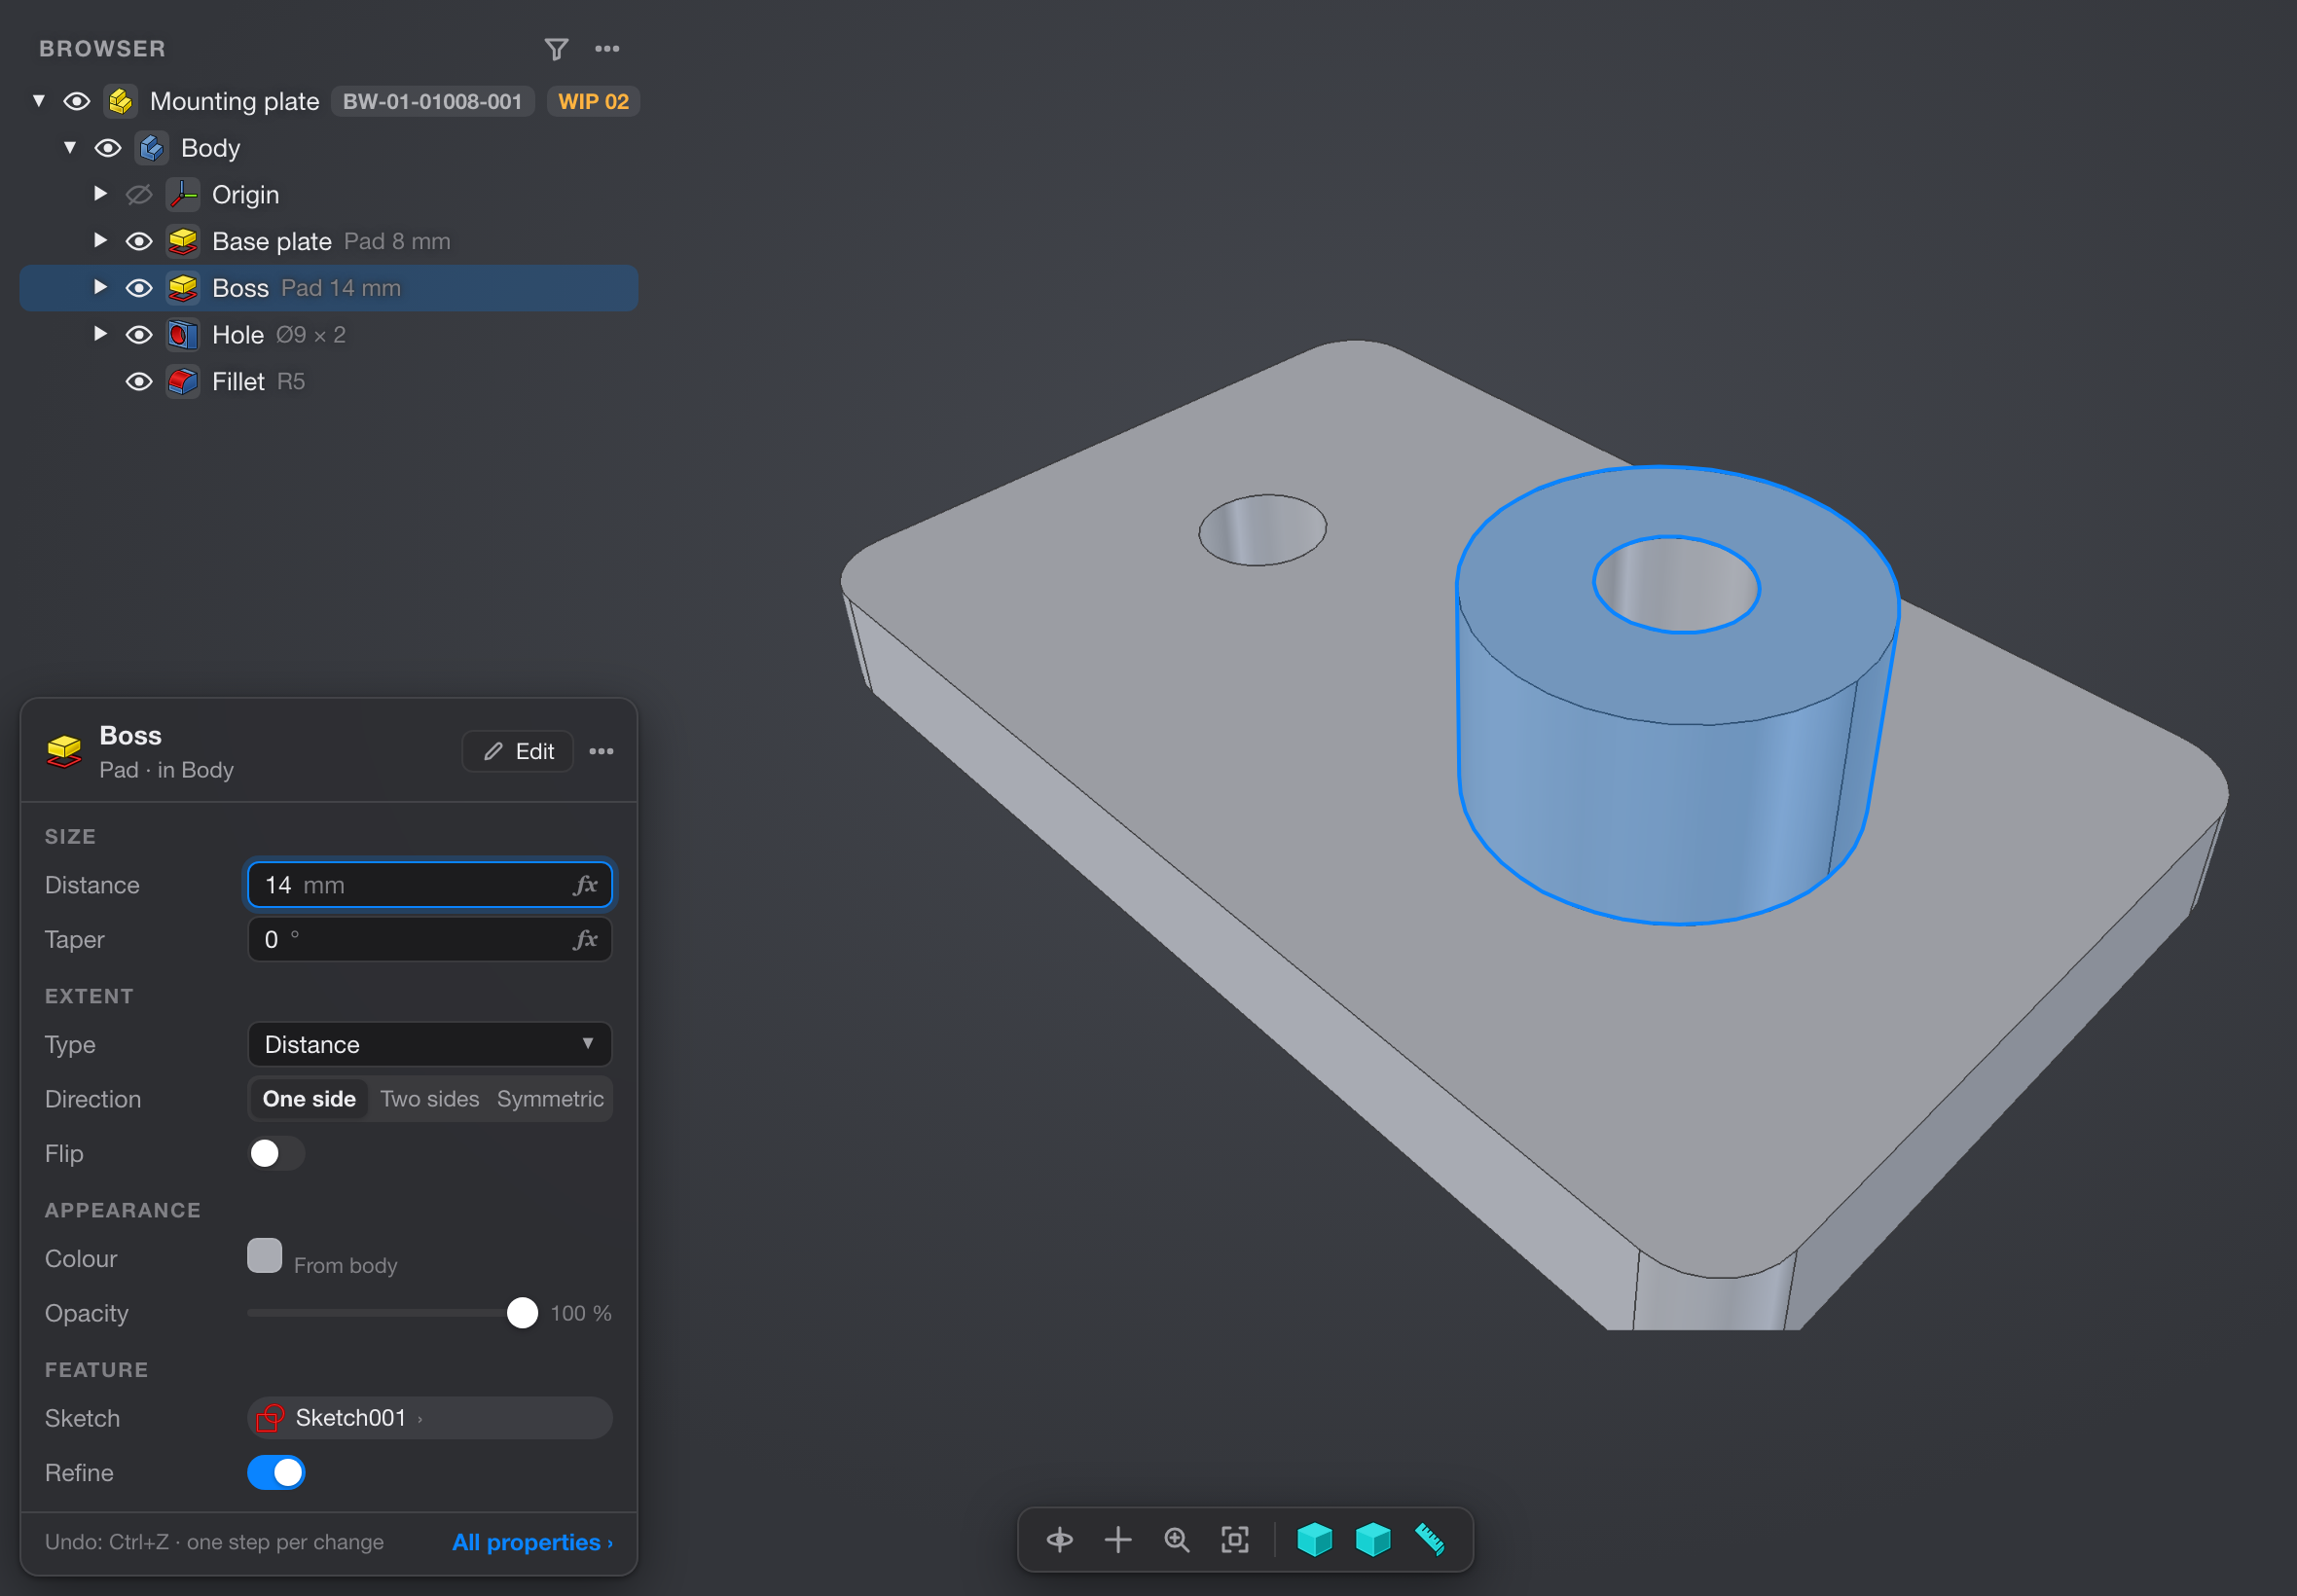
\includegraphics[width=0.75\linewidth]{fig/uix12_browser_dark.png}}{\fbox{uix12\_browser\_dark.png}}
\caption{The same, dark.}
\label{fig:uix12-dark}
\end{figure}

\begin{figure}[!htbp]
\centering
\IfFileExists{fig/uix12_states.png}{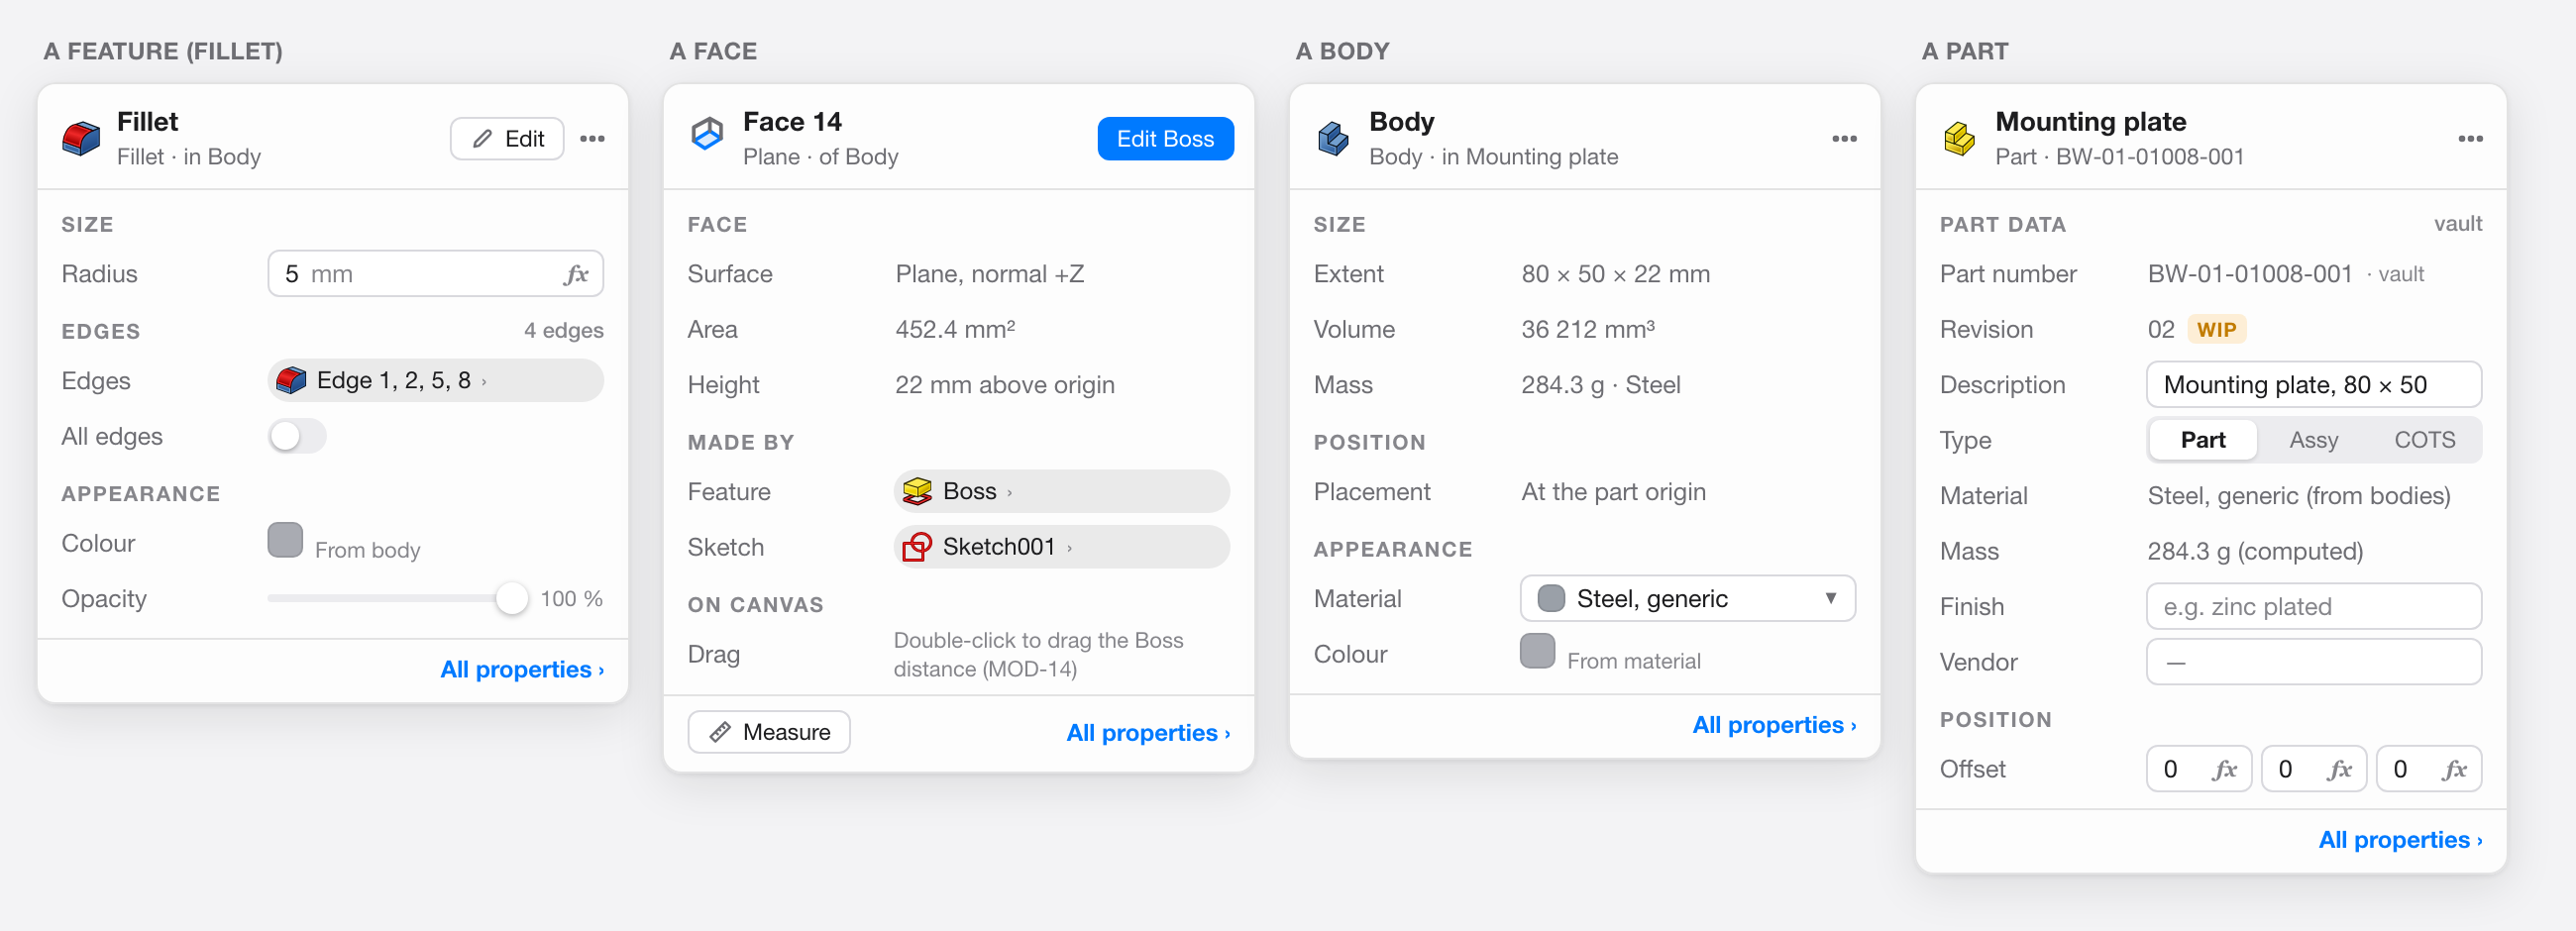
\includegraphics[width=\linewidth]{fig/uix12_states.png}}{\fbox{uix12\_states.png}}
\caption{The four kinds of selection (mock). \emph{Feature:} its size and options. \emph{Face:} what it is, the
feature that made it and its sketch (one click selects them), \emph{Edit Boss}, \emph{Measure}. \emph{Body:} extent,
volume, mass and material. \emph{Part:} the part data from the vault schema (read-only where the vault or a
computation owns the value) and its position.}
\label{fig:uix12-states}
\end{figure}

%----------------------------------------------------------------------
\subsubsection*{1. What the spike showed (23 Oct)}

A script in this build (\file{plan-ui/spike\_inspector.py}, on a copy of your configuration) made a plate with a
boss, a hole and fillets inside a Part carrying the part properties, then put a prototype inspector into the
Browser (figure~\ref{fig:uix12-spike}).
\begin{center}
\small
\begin{tabularx}{\linewidth}{@{}lX@{}}
\toprule
Question & Result\\
\midrule
Where the tabs live & The Browser card is the \emph{Model} dock: a \code{QSplitter} holding the tree and
  \code{Gui::PropertyView}, whose \code{QGridLayout} holds one \code{QTabWidget} (\code{propertyTab}, View and
  Data; \file{Gui/PropertyView.cpp:83}). Python finds it by class name.\\
Replacing them & Taking \code{propertyTab} out of the layout and putting a \code{QStackedWidget} [inspector,
  \code{propertyTab}] in its place \textbf{works}: FreeCAD keeps updating its editor (it holds a pointer, not a
  layout slot), and \code{setCornerWidget} adds the \emph{$\langle$ Inspector} button on the tab bar. No C++.\\
Selection & \code{Gui.Selection.getSelectionEx("", 0)} gives the full path (\code{Part}, \code{"Body.Pad001."});
  \code{obj.getSubObject(sub, retType=1)} resolves it. A face comes as \code{"Body.;\#ad:1;\ldots.Face14"}.\\
Face $\rightarrow$ feature & \code{Body.getElementHistory("Face14", recursive=True, sameType=True)} walks Fillet
  $\rightarrow$ Hole $\rightarrow$ Pad; the last entry is the feature that made the face (\emph{Boss}).
  Correct on every face tried.\\
Property metadata & \code{getTypeIdOfProperty}, \code{getGroupOfProperty}, \code{getEditorMode},
  \code{getPropertyStatus}, \code{getDocumentationOfProperty}, \code{getEnumerationsOfProperty}: everything the
  grouping below needs. PartDesign marks inactive options read-only (\code{Length2} while one-sided), so hiding
  read-only rows makes the card follow the mode for free.\\
Editing & A \code{Gui::QuantitySpinBox} from \code{Gui.UiLoader}, bound with \code{Gui.ExpressionBinding}, gives
  units and the $f(x)$ button. Setting the boss to 20\,mm in one transaction took \textbf{20\,ms} including the
  recompute and left one undo step (``Inspector: Length'').\\
\bottomrule
\end{tabularx}
\end{center}

\begin{figure}[!htbp]
\centering
\IfFileExists{fig/uix12_spike.png}{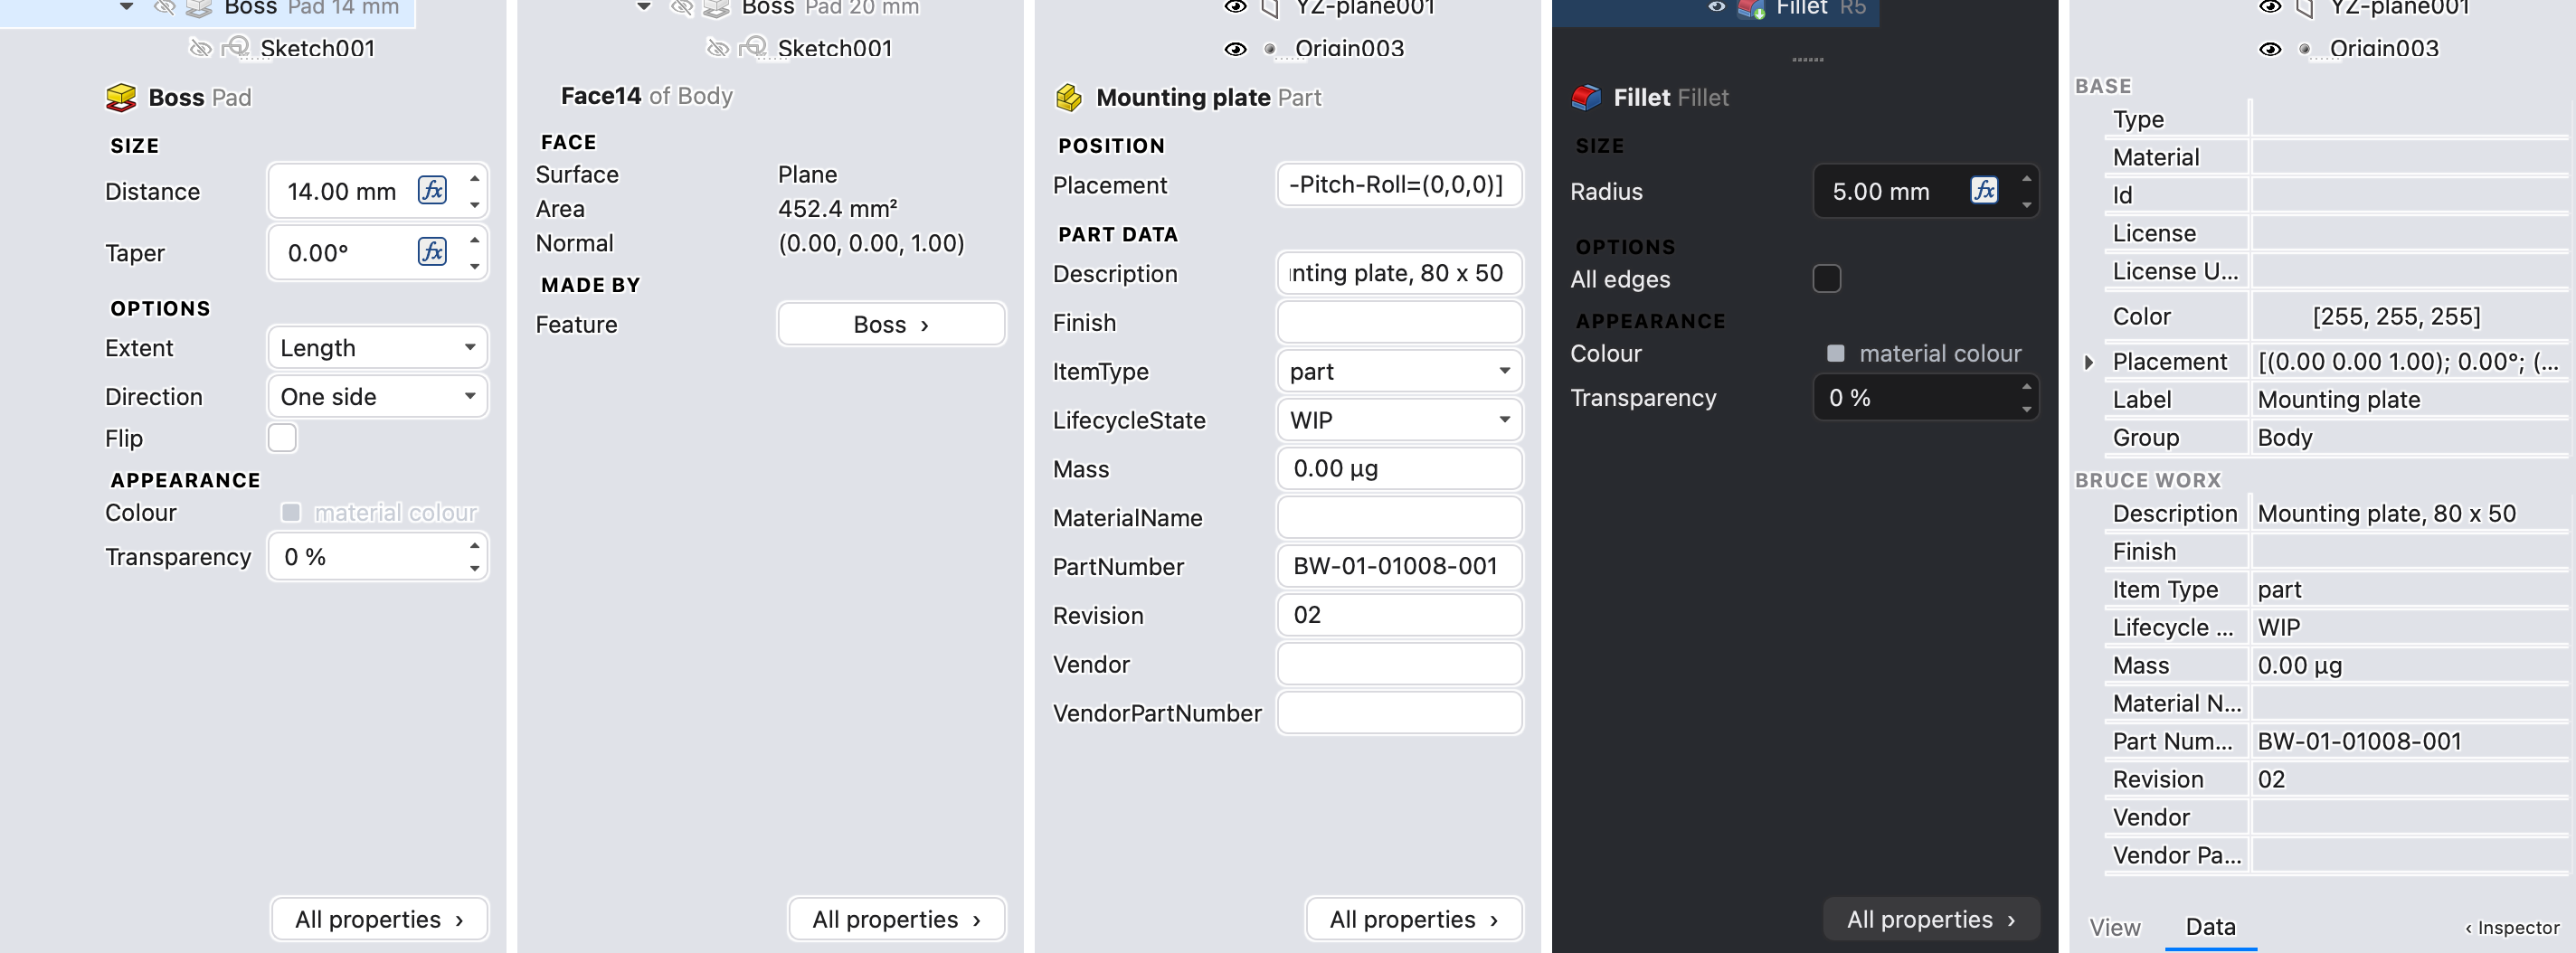
\includegraphics[width=\linewidth]{fig/uix12_spike.png}}{\fbox{uix12\_spike.png}}
\caption{The spike in this build (Browser panel grabs, not a mock): the boss pad, a face traced to \emph{Boss}, the
Part with its Heuretes FreeCAD properties, a fillet in dark mode, and \emph{All properties} with the
\emph{$\langle$ Inspector} button. The look is unstyled; the mock above is the target.}
\label{fig:uix12-spike}
\end{figure}

%----------------------------------------------------------------------
\subsubsection*{2. Theory: which property goes where}

An object $o$ has properties $p$, each with a type $\tau(p)$, a group $\gamma(p)$, an editor mode $m(p)$ and a
name $n(p)$. The inspector shows a property in at most one group $g(p)$, chosen by the \textbf{first rule that
holds}:
\begin{center}
\small
\begin{tabularx}{\linewidth}{@{}clX@{}}
\toprule
\# & Rule & Group\\
\midrule
1 & $\text{Hidden} \in m(p)$, or $n(p)$ starts with \code{\_}, or an internal shape/link & none (full editor only)\\
2 & $(o.\text{TypeId}, n(p)) \in C$, the curated table & as $C$ says, with $C$'s friendly label and order\\
3 & $\text{ReadOnly} \in m(p)$ and $p$ is a feature option & none (an inactive option, e.g.\ \code{Length2} when one-sided)\\
4 & $\gamma(p) = $ the part-property group (\code{BruceWorx}) & \textsc{Part data}, in schema order; read-only when the schema says \code{readonly}\\
5 & $\tau(p) = $ \code{PropertyPlacement}, or $n(p) \in \{$\code{AttachmentOffset}, \code{MapMode}$\}$ & \textsc{Position}\\
6 & $\tau(p) \in$ quantities (Length, Distance, Angle, constrained quantities) & \textsc{Size}\\
7 & $\tau(p) \in \{$Enumeration, Bool$\}$, $\gamma(p) \notin \{$Base, Attachment$\}$ & \textsc{Options}\\
8 & $\tau(p) \in$ links (Profile, Base) & \textsc{Feature}, as chips\\
9 & otherwise & none\\
\bottomrule
\end{tabularx}
\end{center}
\textsc{Appearance} comes from the view object, not the data: \code{ShapeAppearance} (colour), \code{Transparency}
(shown as opacity) and, for bodies, the material. The groups always come in the order \textsc{Size},
\textsc{Options}, \textsc{Position}, \textsc{Appearance}, \textsc{Part data}, \textsc{Feature}. The curated table $C$
covers the twenty or so types used daily (Pad, Pocket, Revolution, Groove, Hole, Fillet, Chamfer, Draft, Thickness,
Mirror and the patterns, Body, Part, Sketch, the primitives, the assembly joints); rules 3--9 cover the rest, so an
unknown type still gets a sensible card. On the Pad, rules 3--9 alone keep 11 of its 37 properties (including
expert ones such as \code{FuzzyTolerance} and \code{AllowMultiFace}); the curated table cuts that to the 7 a user
needs (figure~\ref{fig:uix12-notes}). On the Fillet the rules alone give 4 rows (Radius, All edges, Refine and the expert \code{FuzzyTolerance}).

\paragraph{One step per change.} Every edit runs in its own transaction (\code{openTransaction} /
\code{commitTransaction}), named after the field, so \texttt{Cmd-Z} undoes exactly one change and the toast of
\eref{UIX-10} can name it. A typed value is applied on Enter or on leaving the field, not per keystroke.

\paragraph{Several objects.} When everything selected has the same type, a row is shown when the property exists on
all of them; equal values are shown, different ones as ``mixed''. One edit sets all of them in one transaction (two
fillets to R3 in one step). Mixed types show only a count and \emph{All properties}.

\paragraph{Staying current.} The card listens to document changes the way FreeCAD's property view does
(\code{signalChangedObject}, recompute, undo/redo) and refreshes on the next event-loop turn, so a drag in the view
(\eref{MOD-14}) or an undo is reflected at once.

%----------------------------------------------------------------------
\subsubsection*{3. In the window}

\begin{itemize}[nosep]
  \item \textbf{Placement.} The inspector takes the lower part of the Browser column; the splitter between tree and
        inspector stays and its position is remembered. In the transparent Browser the inspector is a frosted card
        (editors need a background); the tree above it keeps its halo.
  \item \textbf{Nothing selected.} The card shows the active part (question~2).
  \item \textbf{Switch.} Preferences $\rightarrow$ BruceWorx $\rightarrow$ \emph{Property inspector in the Browser}
        (default on); off brings back the stock View/Data tabs.
  \item \textbf{Style.} Group captions in the existing small-caps style (\code{BrowserGroupCaptions}), fields and
        switches from \file{BruceWorx.qss} tokens, light and dark.
\end{itemize}

%----------------------------------------------------------------------
\subsubsection*{4. Build order and effort}

\begin{center}
\small
\begin{tabularx}{\linewidth}{@{}lXl@{}}
\toprule
\# & Step & Effort\\
\midrule
1 & Embed (stack in place of the tabs, \emph{All properties} and back), preference, remembered state & 0.5\,d\\
2 & Grouping rules and the curated table, pure Python with unit tests & 1\,d\\
3 & Editors: unit fields with expressions, segmented choices, switches, link chips, colour and opacity, placement;
    one transaction each & 1.5\,d\\
4 & Face, body and part cards: face facts, the feature that made it, extent/volume/mass, part data with the
    schema's read-only rules & 1\,d\\
5 & Multi-selection, live refresh, undo, styling light and dark & 1\,d\\
6 & Checklist (Pad, Pocket, Fillet from the inspector), tests, screenshots, write-up & 0.5\,d\\
\midrule
 & Total & 5.5\,d\\
\bottomrule
\end{tabularx}
\end{center}
\textbf{Feasibility: Python only} (a new \file{bruceworx\_inspector.py}, an install call, a preference and a QSS
block). \textbf{Risks.} FreeCAD code that later assumes \code{propertyTab} sits directly in the layout (none today;
a \code{[BW]} hook in \file{PropertyView.cpp} is the fallback). Very large selections (a thousand objects) need the
multi-selection pass capped. The Nxt-style transparent tree over a busy model can make the frosted card the only
readable part; the card's opacity is a token.

%----------------------------------------------------------------------
\subsubsection*{Built (24 Oct)}

Your answers to the six questions below (24 Oct): friendly labels with FreeCAD's name as the tooltip; \textbf{an
empty card} when nothing is selected (a one-line hint, not the active part); the frosted card; \textbf{body position
editable} (as parts and components); several objects of one type edited together in one undo step; \emph{Sketch on
face} now, \emph{Offset face} with \eref{MOD-04}.

\begin{figure}[!htbp]
\centering
\IfFileExists{fig/uix12_built_light.png}{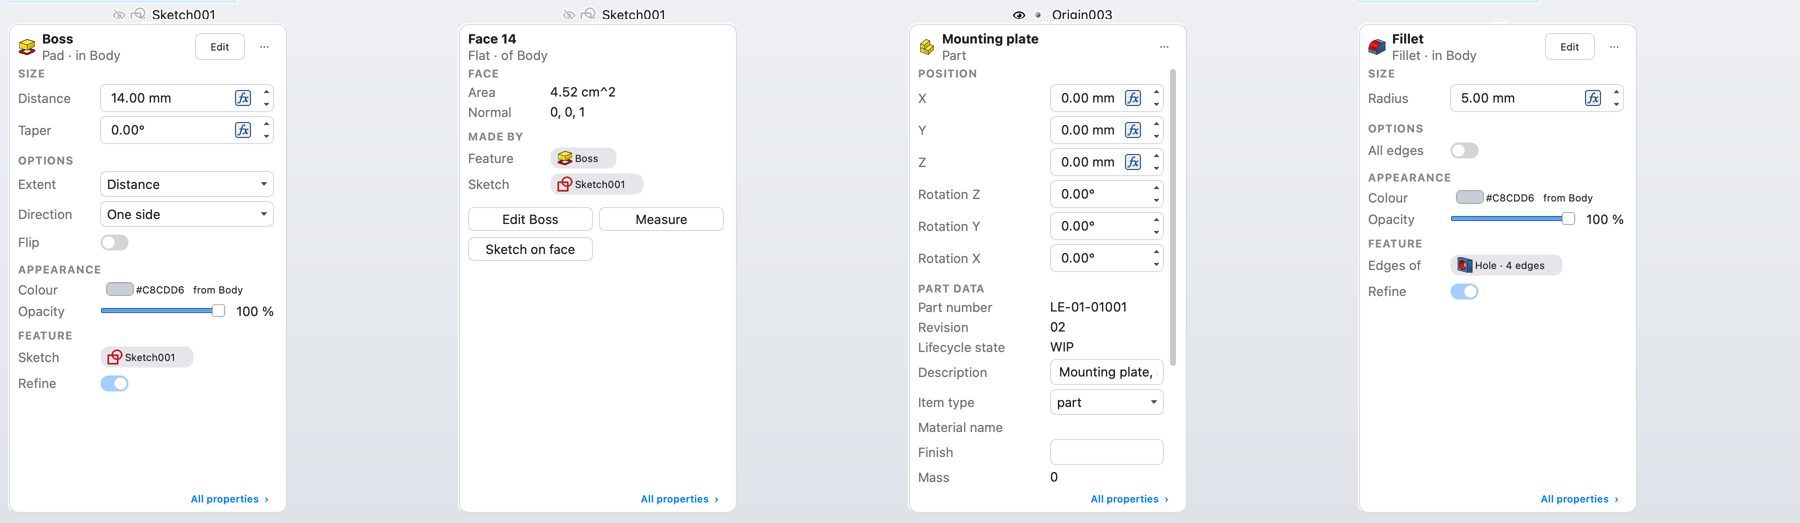
\includegraphics[width=\linewidth]{fig/uix12_built_light.png}}{\fbox{uix12\_built\_light.png}}\\[4pt]
\IfFileExists{fig/uix12_built_dark.png}{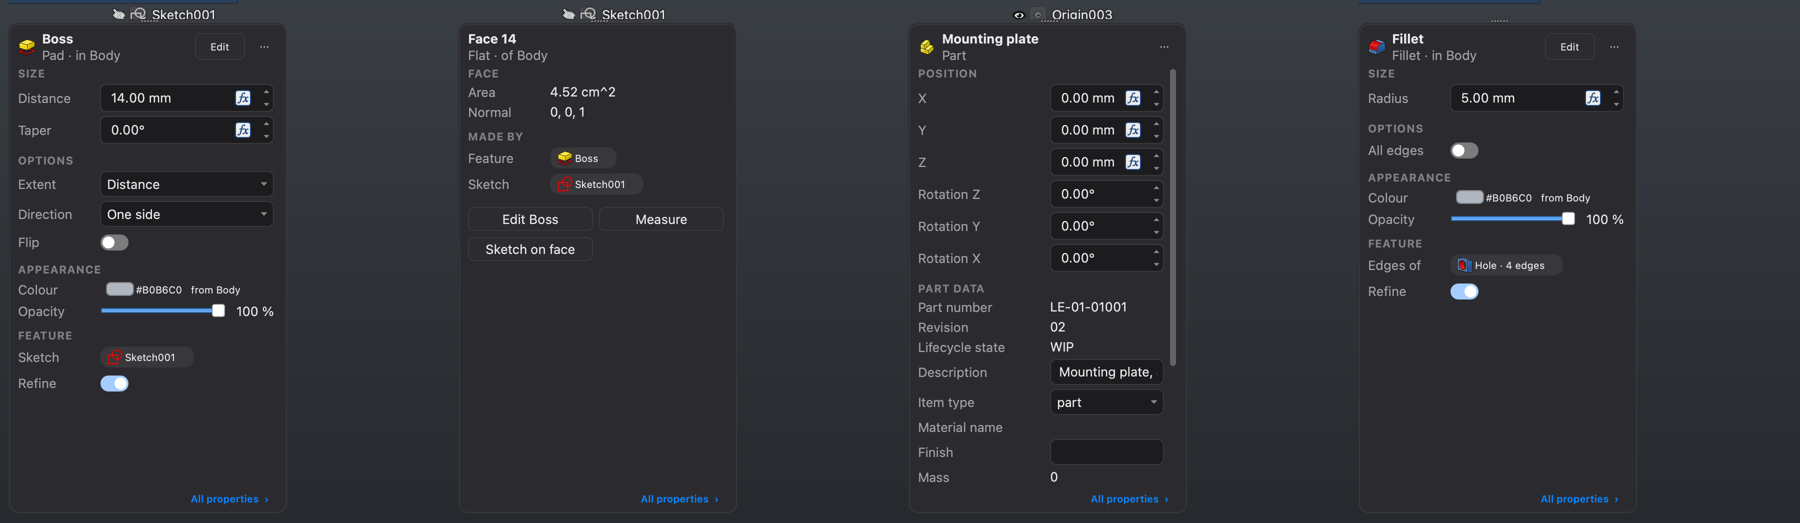
\includegraphics[width=\linewidth]{fig/uix12_built_dark.png}}{\fbox{uix12\_built\_dark.png}}
\caption{The inspector as built, light and dark (Browser panel grabs on a configuration copy): the Boss pad, a face
traced to Boss with \emph{Edit Boss}, \emph{Measure} and \emph{Sketch on face}, the Part with its part data, the
fillet with its edges as a chip.}
\label{fig:uix12-built}
\end{figure}

\file{src/Mod/BruceWorx/bruceworx\_inspector.py} (Python only), installed from \file{InitGui.py}; the switch is
Preferences $\rightarrow$ BruceWorx $\rightarrow$ \emph{Property inspector in the Browser}; styles in
\file{BruceWorx.qss}; tests \file{TestBruceWorxInspector.py} (21, the grouping rules and the curated table).
\begin{itemize}[nosep]
  \item FreeCAD's \code{propertyTab} moves into a stack beside the card; \emph{All properties} and
        \emph{$\langle$ Inspector} switch between them and the choice is remembered, as is the splitter position.
        Switching the preference off gives the tabs back at once.
  \item Choices: a segmented control when there are at most three short ones (18 characters in all, so they fit a
        narrow Browser), otherwise a menu. Pad's \emph{Direction} (One side, Two sides, Symmetric) is therefore a menu.
  \item A feature's colour and opacity are its body's (PartDesign gives all features the body's look); the row says
        ``from Body''. A body or a Part gets extent, volume, mass and material, with \emph{Material\ldots}.
  \item Measured in the check run: setting the boss to 20\,mm took 21\,ms with the recompute, one undo step
        ``Boss: Distance''; switching to two sides shows \emph{Distance~2} and \emph{Taper~2}; undo reverts only that
        step and the card follows; two pads set to 6\,mm in one step ``2 objects: Distance''.
  \item Joints and the less common PartDesign features use the rules (no curated rows yet).
\end{itemize}

%----------------------------------------------------------------------
\subsubsection*{Questions before UIX-12 starts}

\begin{enumerate}
  \item \textbf{Labels.} Friendly names (``Distance'', ``Extent'') or FreeCAD's property names (``Length'',
        ``Type'')?\\
        \emph{Recommendation:} friendly names, with FreeCAD's name as the tooltip so the Data tab stays easy to find.
  \item \textbf{Nothing selected.} Show the active part's card, or an empty card?\\
        \emph{Recommendation:} the active part: part number, revision, mass at a glance.
  \item \textbf{Transparent Browser.} The inspector on a frosted card (mock), or transparent like the tree?\\
        \emph{Recommendation:} frosted card.
  \item \textbf{Body position.} In PartDesign a body normally stays at the part origin. Show its placement
        read-only (mock) or editable?\\
        \emph{Recommendation:} read-only for bodies, editable for parts and assembly components.
  \item \textbf{Several selected.} Edit all objects of one type together in v1?\\
        \emph{Recommendation:} yes, one undo step.
  \item \textbf{Face card actions.} Besides \emph{Edit <feature>} and \emph{Measure}: also \emph{Sketch on face}
        and \emph{Offset face} (\eref{MOD-04}) later?\\
        \emph{Recommendation:} \emph{Sketch on face} now (it is one command), \emph{Offset face} with MOD-04.
\end{enumerate}

%----------------------------------------------------------------------
\subsubsection*{Redesign (24 Oct): a tabbed panel on the right, for approval}

You tried the card in the Browser on 24 Oct (after a macOS layout bug that pushed it 230\,px to the right was
fixed) and found it \emph{too tall, with big fields, and properties that add little}; look at how commercial
software shows properties, and make it \emph{a tab in the window on the right where we can choose between
options}. Your answers (24 Oct):
\begin{center}
\small
\begin{tabularx}{\linewidth}{@{}lX@{}}
\toprule
Question & Answer\\
\midrule
Style & Fusion's dialog style: labels left, compact fields right, folding sections, only key values open.\\
Tabs on the right & \textbf{Properties}, \textbf{Vault}, \textbf{Parameters}, \textbf{Physical}.\\
A selected feature & Its 2--4 key values and \emph{Edit}; the rest under \emph{More}; then the part it belongs to.\\
A command (Pad\ldots) & \textbf{Its own tab}, chosen when the command opens; you can flip to another tab mid-command.\\
The Browser & \textbf{Keeps FreeCAD's View/Data tabs} under the tree (the card leaves the Browser).\\
\bottomrule
\end{tabularx}
\end{center}

\paragraph{How commercial tools do it.} None of them puts a feature's full parameter grid in a side panel.
SolidWorks and Fusion edit a feature in its own dialog (PropertyManager, the command dialog); what they show as
\emph{properties} is the \emph{item}: identity (part number, description, revision), material and appearance, and
physical properties (Fusion's \emph{Properties} and SolidWorks' \emph{Mass Properties}: mass, volume, area, centre
of mass, inertia). Onshape and Inventor keep identity, material and appearance in a panel on the right. Fusion's
\emph{Change Parameters} is the one place where every dimension of the model is listed, with user parameters and
expressions. The redesign follows that split: the \textbf{Properties} tab is about the selected item (with a feature's
few key values, as you chose), \textbf{Physical} about its mass properties, \textbf{Parameters} about the dimensions.

\begin{figure}[!htbp]
\centering
\IfFileExists{fig/uix12_right_tabs_light.png}{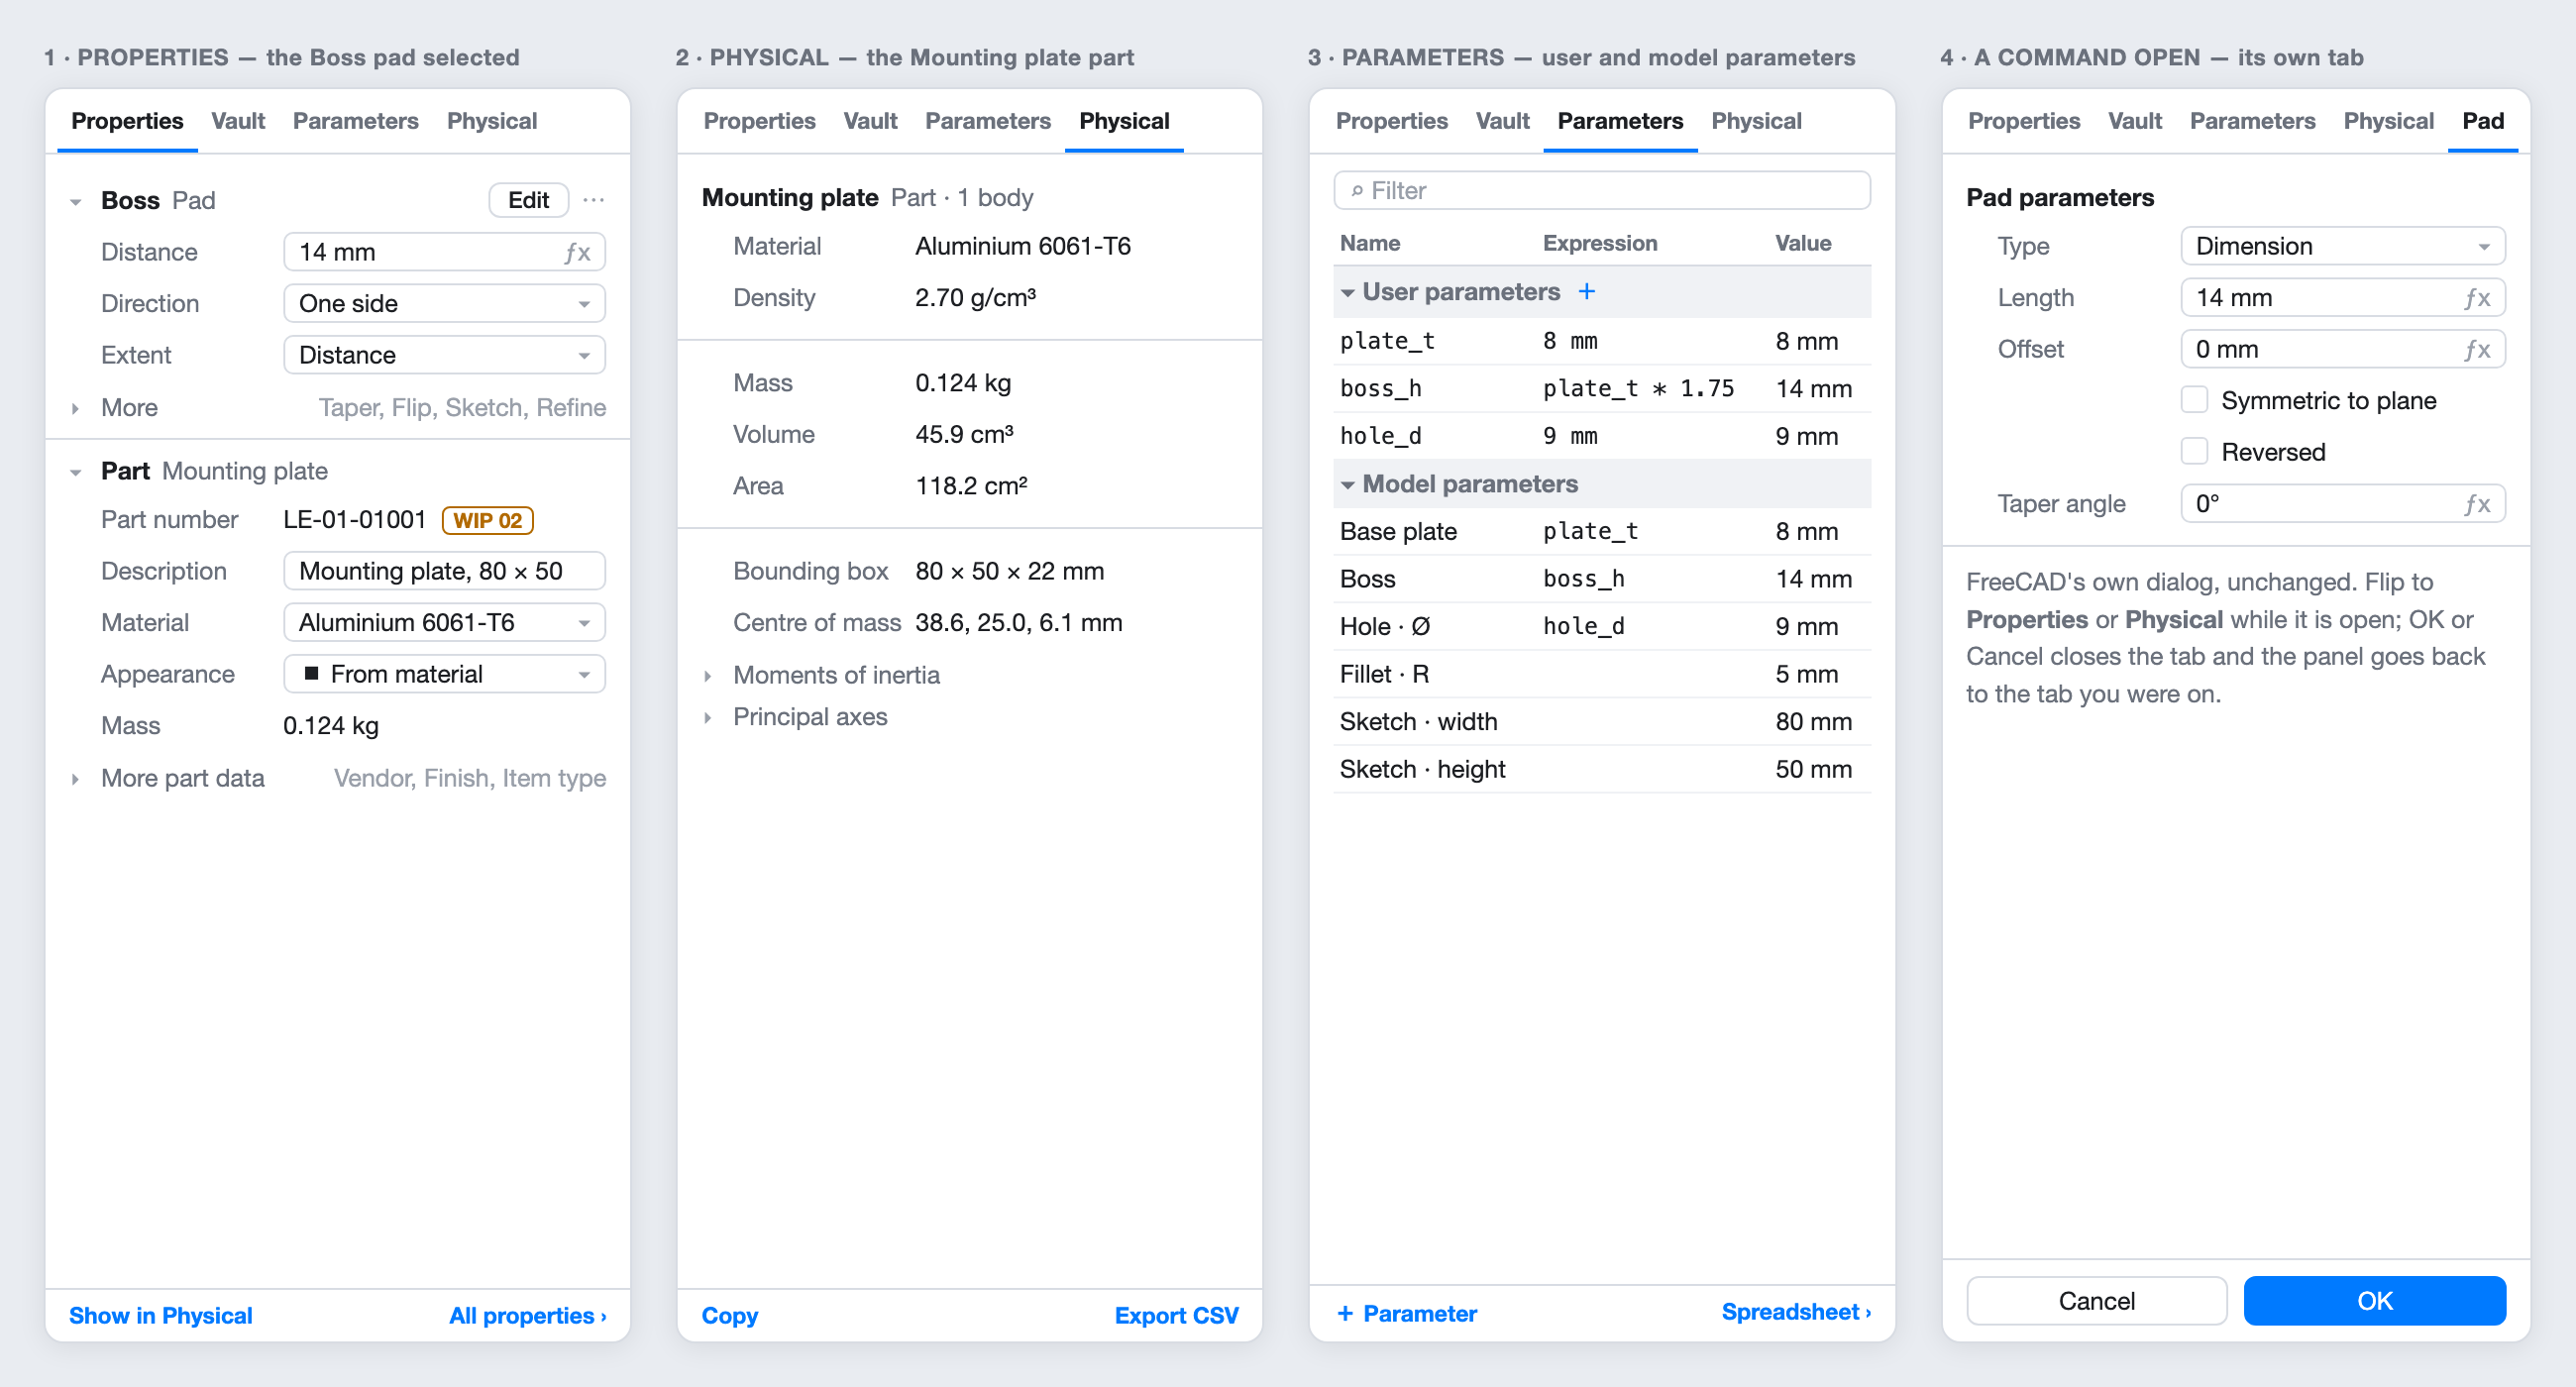
\includegraphics[width=\linewidth]{fig/uix12_right_tabs_light.png}}{\fbox{uix12\_right\_tabs\_light.png}}\\[4pt]
\IfFileExists{fig/uix12_right_tabs_dark.png}{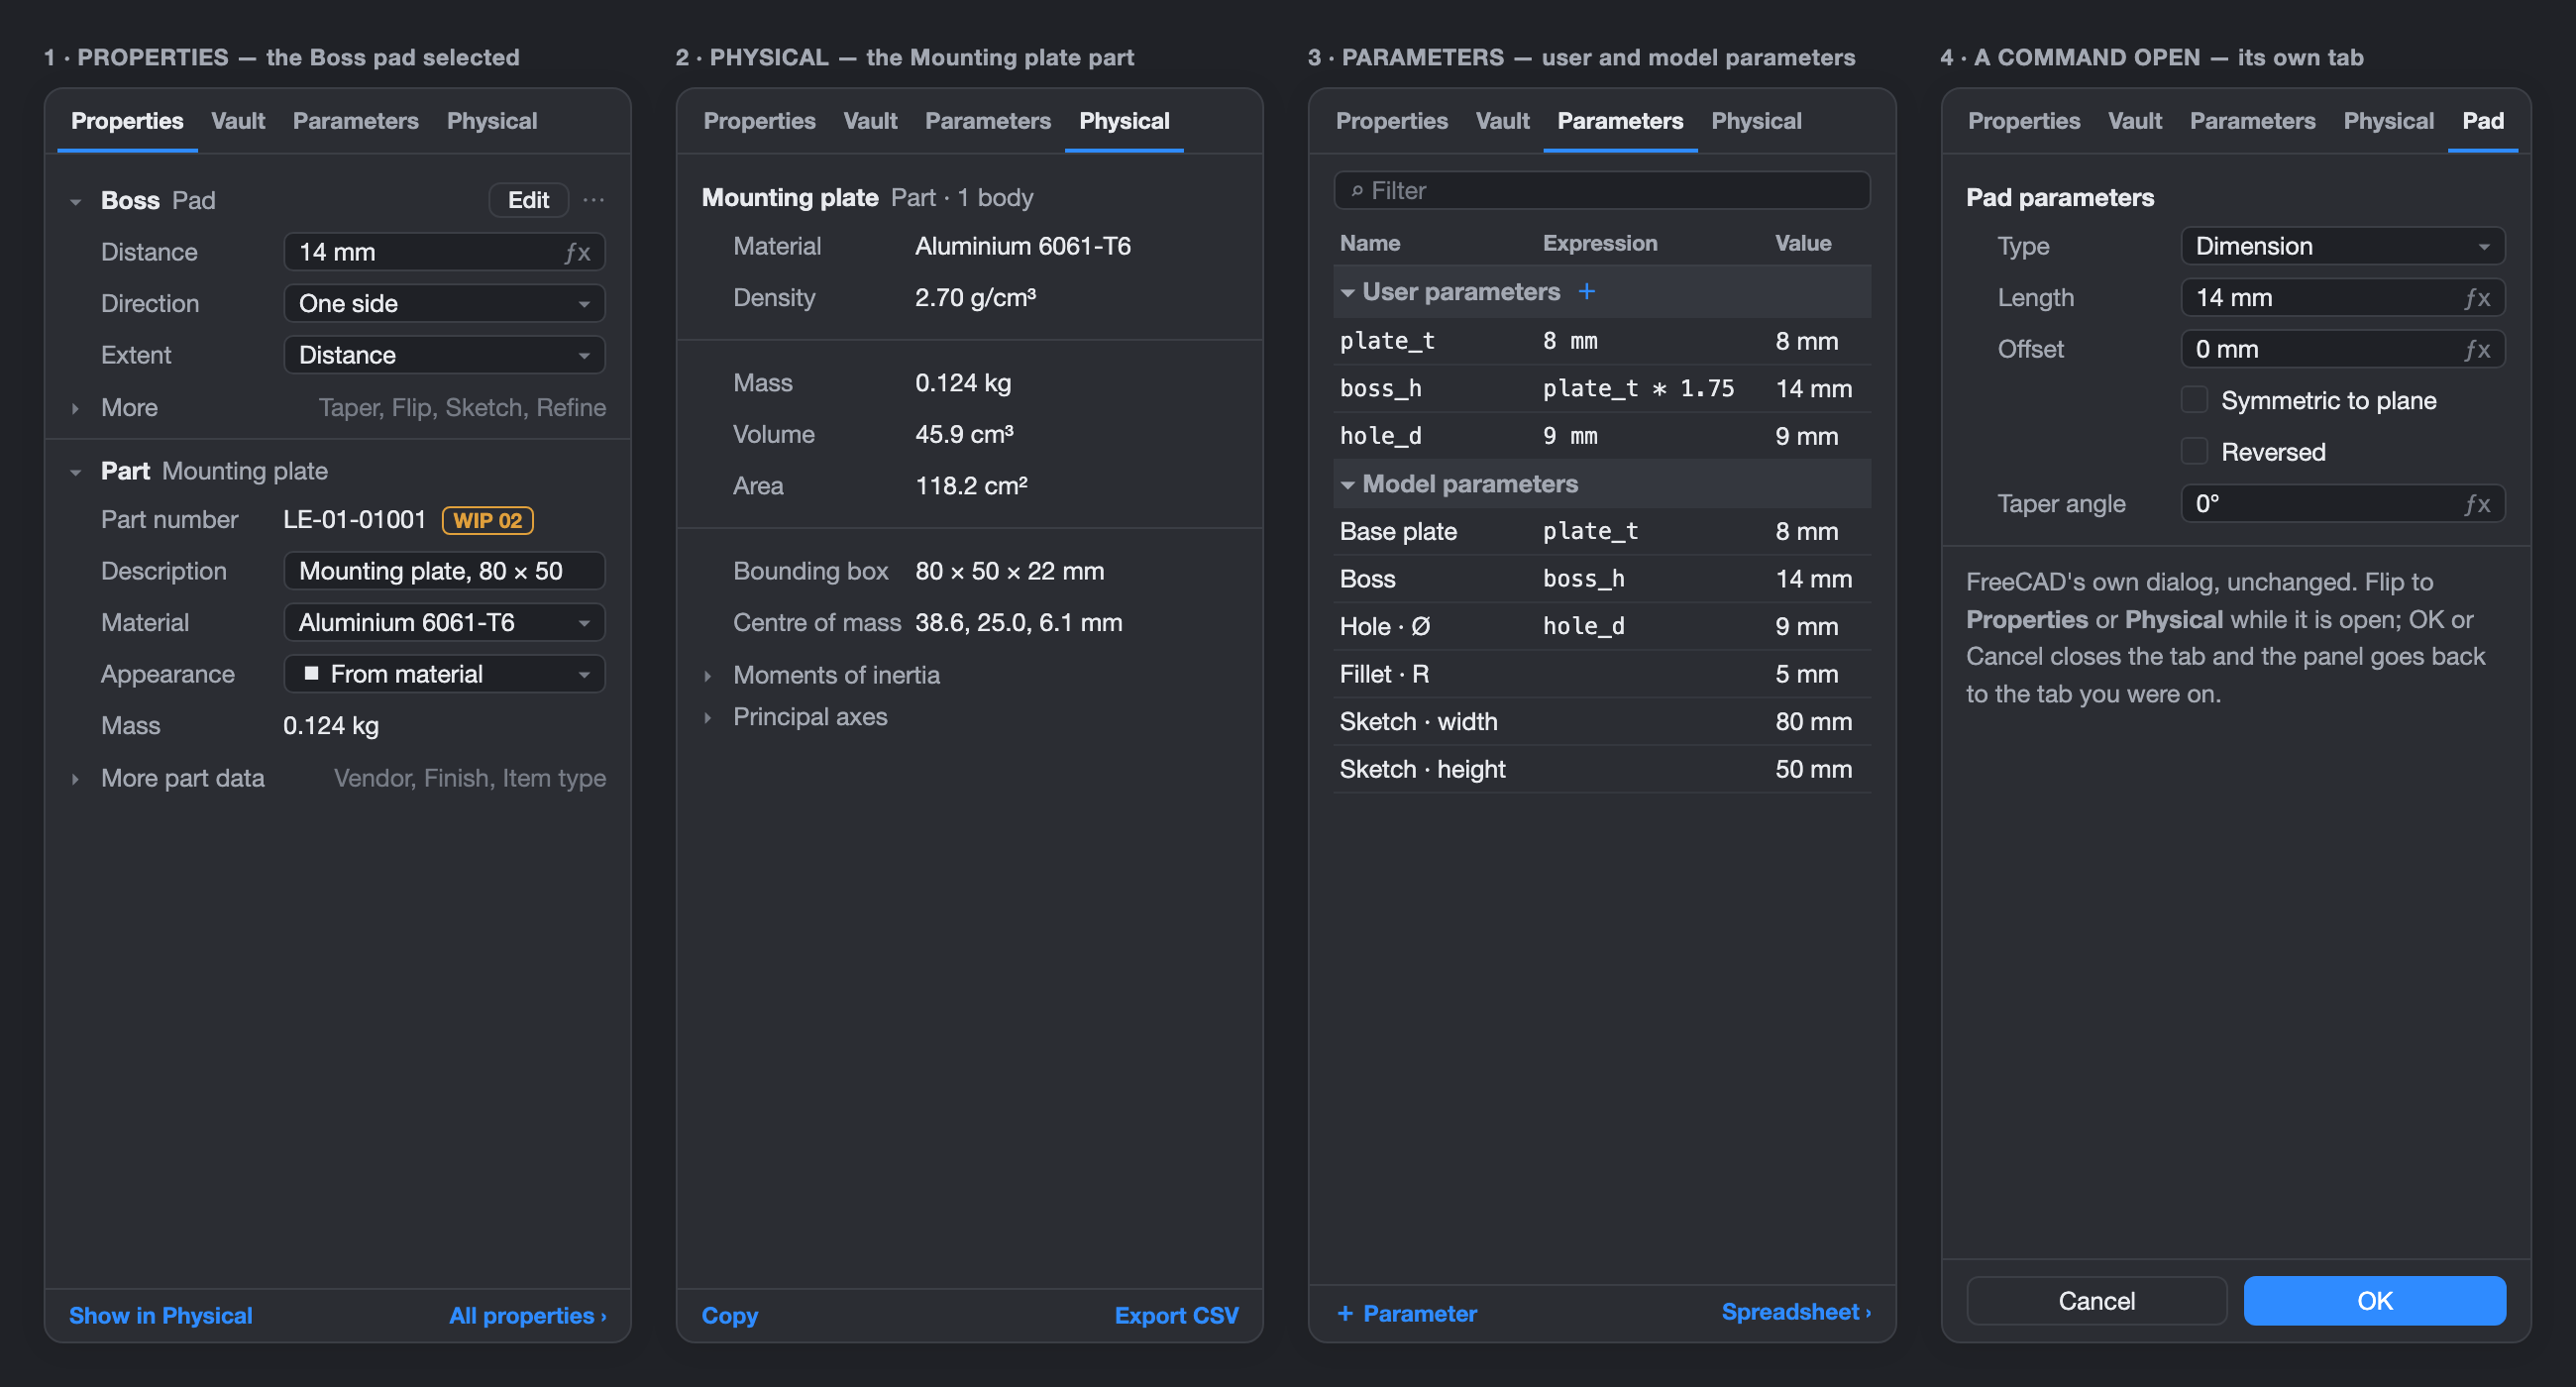
\includegraphics[width=\linewidth]{fig/uix12_right_tabs_dark.png}}{\fbox{uix12\_right\_tabs\_dark.png}}
\caption{The right panel with its tabs (mock, light and dark). 1: Properties with the Boss pad selected (key values,
\emph{More} folded, then the part). 2: Physical for the part. 3: Parameters, user parameters above the model's
dimensions. 4: a command open: FreeCAD's Pad dialog in its own tab.}
\label{fig:uix12-right-tabs}
\end{figure}

\paragraph{What it takes (read from FreeCAD's code, 24 Oct).} The right panel is FreeCAD's overlay panel
\code{OverlayRight}, a tab widget over docks; today it holds only the \emph{Tasks} dock and hides while no command is
open (our \code{[BW]} rule in \code{OverlayTabWidget::checkAutoHide} applies when it holds that dock alone). With
more docks in it, it stays up and shows a tab per dock, and FreeCAD already brings the Tasks tab forward when a
dialog opens and folds it when the dialog closes (\code{OverlayManager::onTaskViewUpdate}) --- the behaviour you
chose. A dock joins the panel only when it is registered through FreeCAD's \code{DockWindowManager}, which Python
cannot reach; one \code{[BW]} function in \file{ApplicationPy.cpp} (\code{FreeCADGui.addDockWindow(name, widget,
area)}, about 30 lines) closes that gap. Everything else is Python: the four tab widgets, reusing the inspector's
grouping rules and editors, made compact; the Vault card moves into its tab.

\begin{center}
\small
\begin{tabularx}{\linewidth}{@{}lXl@{}}
\toprule
\# & Step & Effort\\
\midrule
1 & \code{[BW]} \code{addDockWindow}; the four docks in \code{OverlayRight}; the Tasks tab named after the command;
    remembered tab and width; the Browser gets its stock tabs back & 1\,d\\
2 & Properties: folding sections, compact fields (no spin arrows; $f(x)$ on hover), key values per type, \emph{More},
    the part section (identity, material, appearance, mass), several objects & 2\,d\\
3 & Physical: mass, volume, area, bounding box, centre of mass; inertia and principal axes folded; Copy, CSV & 1\,d\\
4 & Parameters: user parameters (add, rename, expression), model dimensions by feature, filter, edits as one
    undo step each & 2.5\,d\\
5 & Vault: the Vault card's panel in its tab; the status-bar button and Cmd-K open the tab & 0.5\,d\\
6 & Styling light and dark, tests, the checklist (Pad, Pocket, Fillet), write-up & 1\,d\\
\midrule
 & Total & 8\,d\\
\bottomrule
\end{tabularx}
\end{center}

\paragraph{Your answers to the questions below (24 Oct).} 1: user parameters in a \textbf{spreadsheet}
(aliases), not a VarSet. 2: the Parameters tab lists \textbf{every} dimension, named or not. 3: a new selection
\textbf{brings Properties forward, unless a feature is being edited} (a command's tab stays in front). 4: the panel
is shown, its width remembered, Cmd-I hides and shows it. 5: the floating Vault card is retired. 6: inertia about
the centre of mass, with a switch for the origin. Building started 24 Oct.
Answer~1 made precise the same evening: \textbf{one} spreadsheet \emph{Parameters} at the root of the top-assembly
file holds every dimension and spec, with a \emph{Used in} column naming the part or drawing each value drives;
every part's dimensions are tied to it by expressions, so changing the sheet updates the model, and the design
worksheet (\eref{MOD-15}, \S\ref{sec:mod15-plan}) reads and writes that sheet.

\paragraph{Built (24 Oct, evening).} The right panel (\file{bruceworx\_rightpanel.py}) carries its tabs, and the
\textbf{Properties} tab is built. The \textbf{Physical} and \textbf{Parameters} tabs are \textbf{paused half-built}:
\file{bruceworx\_physical.py} and \file{bruceworx\_parameters.py} are in the tree but not installed
(\code{InitGui.\_BW\_PAUSED}); when it resumes, the Parameters tab follows the one-sheet decision above (today it
makes a \emph{Parameters} sheet in each document). At your request \emph{Create Vault} now opens as a
\textbf{full-window tab} of its own (numbered sections, Cancel / Create at the bottom; a switch on Preferences
$\rightarrow$ BruceWorx gives the right-panel version back). The document tabs sit at the \textbf{bottom or top}
(Preferences $\rightarrow$ BruceWorx $\rightarrow$ \emph{Document tabs}, default bottom), and the Start page is
\textbf{pinned as the first tab}, without a close button (\file{bruceworx\_doctabs.py}, switch \code{PinStartTab}).

\paragraph{Questions before the redesign is built.}
\begin{enumerate}
  \item \textbf{User parameters: where do they live?} In a FreeCAD~1.0 \code{App::VarSet} named \emph{Parameters} in
        each document (typed, expressions, shows in the tree), or in a spreadsheet (aliases)?\\
        \emph{Recommendation:} a VarSet; \emph{Spreadsheet~$\rangle$} stays for tables.
  \item \textbf{Model parameters: which dimensions?} Every feature dimension plus \emph{named} sketch constraints, or
        also unnamed sketch dimensions?\\
        \emph{Recommendation:} features and named constraints; unnamed ones behind a ``Show all sketch dimensions''
        switch.
  \item \textbf{Following the selection.} Should selecting something switch to the Properties tab, or stay on the
        tab you chose (Physical then shows the new selection)?\\
        \emph{Recommendation:} stay on your tab; every tab follows the selection.
  \item \textbf{The panel while no command is open.} Always shown (it takes about 300\,px of the view), or hidden
        until you open it (a button in the title row and a shortcut)?\\
        \emph{Recommendation:} shown, its width remembered; Cmd-I hides and shows it.
  \item \textbf{The Vault card.} Retire the floating Vault card once the Vault tab exists?\\
        \emph{Recommendation:} yes; one place for the vault.
  \item \textbf{Inertia units and frame.} Moments of inertia about the centre of mass in kg$\cdot$mm$^2$, or about the
        part origin?\\
        \emph{Recommendation:} about the centre of mass, in the document's units, with a switch for the origin.
\end{enumerate}
